%% Springer Nature journal article
%% Class: sn-jnl with Vancouver numbered reference style
\documentclass[pdflatex,sn-vancouver-num,Numbered]{sn-jnl}

\usepackage{graphicx}
\usepackage{multirow}
\usepackage{booktabs}
\usepackage{array}
\usepackage{amsmath}
\usepackage{url}
\usepackage{orcidlink}
\usepackage[numbers,sort&compress]{natbib}

\raggedbottom

\begin{document}

\title[Measurement Error in Sole-Supplier Drug Markets]{When a sole supplier is not sole: duplicate market keys, misclassified exits, and what survives both in US Medicaid drug markets}

\author*[1]{\fnm{Vasu} \sur{Atmakuri}\,\orcidlink{0009-0007-5955-2466}}\email{athmakurivasu@gmail.com}

\author[1]{\fnm{Souseelya} \sur{Kidambi}\,\orcidlink{0009-0003-9788-8949}}\email{souseelyakidambi.res@gmail.com}

\affil[1]{\orgname{Independent Researcher}, \city{Dallas}, \state{TX}, \country{USA}}

\abstract{\textbf{Background.} Concern about single-source drug markets rests on counting
suppliers within a market defined by active ingredient and dosage form. Both halves of that
procedure can fail. The market key is built from a free-text ingredient string that is not
normalised, and an observed supplier exit need not be a supply disruption.

\textbf{Methods.} We built a national quarterly panel of Medicaid State Drug Utilization Data
from 2016Q1 to 2026Q1 and detected labeler exits as a sustained fall to under five percent of a
labeler's own prior dispensing. We then did two things that prior work using this market
definition has not. First, we defined the market by route of administration as well as dosage form, and
normalised the ingredient key, collapsing strings that differ only in form nouns,
strengths, word order or salt naming. The merges were then validated against FDA
structured active-ingredient data, which is populated independently of the free-text
name the key is built from. Second, we audited every
sole-labeler exit against FDA withdrawal notices, prescription-to-over-the-counter switch
approvals, FDA and ASHP shortage records and recall filings, classifying each as a supply
disruption, a non-supply event, or undetermined. Replacement by remaining labelers was measured
with a ratio that is not mechanically fixed by the event definition, and recovery was measured
as time from a market's first threshold crossing to its first restoration, with censoring.

\textbf{Results.} Dosage form alone does not identify a market: the form string
``solution'' covers 1{,}727 oral products, 1{,}017 topical, 325 ophthalmic and 50 otic, and in
the original bucketing every eye and ear product was filed as an oral liquid. Using route as
well as form, and then normalising the ingredient key, 424 of 3{,}294 keys prove to be
duplicates of another key, leaving 2{,}870 markets; FDA substance data confirms 305 of 316
testable merges (96.5 percent). Six of twenty apparent sole-labeler exits are not sole-labeler
exits at all. In the clearest case a firm holding 6.4 percent of a nineteen-labeler pregabalin
market had been recorded as its sole supplier. Of the thirteen that remain, three are not supply
disruptions: the market-wide withdrawal of ranitidine and two prescription-to-over-the-counter
switches. Three are documented supply disruptions, two of them the same recall episode, and
seven could not be classified. The concentration gradient survives the corrections: median
replacement ratios are 1.77 where the departing share was under 35 percent, 0.82 at 65 to 95
percent and 0.00 at 95 percent or more, and sole-labeler markets collapse below two percent of
baseline dispensing at 38.5 percent against 0.0 percent among 325 matched risk-set control
observations, a risk difference of 38.5 points (95\% CI 15.4 to 61.5). Measured from first
crossing with censoring, sole-labeler markets are slower to regain 90 percent of baseline
(log-rank $p=0.056$). The zero-replacement result, however, is concentrated in events whose
cause could not be established: among the three documented supply disruptions the median
replacement ratio is 0.24.

\textbf{Conclusions.} Supplier counts in these data are inflated by a measurement artefact that
operates before any supplier is counted, and apparent sole-supplier exits are frequently
regulatory or commercial rather than supply events. The association between pre-exit
concentration and dispensing loss is robust to both corrections. Claims that such markets fail to
replace after a supply disruption are not supported by the subset in which a supply disruption
can actually be documented.}

\keywords{drug shortages, generic drug markets, market definition, measurement error, Medicaid,
pharmaceutical supply chain, supplier concentration}

\maketitle

\section{Introduction}\label{sec:intro}

Policy concern about the resilience of US generic drug supply is usually expressed as a count.
The Food and Drug Administration's root-cause analysis of shortages reports the share of markets
served by a small number of manufacturers \cite{fda2019taskforce}; structural work on generic
entry estimates how manufacturing complexity and regulatory cost hold that number down
\cite{wang2023}; and descriptive work on the generic landscape tracks how many sellers a molecule
has over time \cite{berndt2017,conti2020}. Reimbursement policy has been linked to shortage
incidence through the same lens \cite{yurukoglu2017}, and the harms of shortages to patients are
well documented \cite{phuong2019,aronson2023}.

Counting suppliers requires first defining the market they supply. The convention, following
Berndt and colleagues, is an active ingredient paired with a dosage form \cite{berndt2017}.
Colazo \cite{colazo2026} has recently argued that supplier counts drawn this way record
administrative visibility rather than operational redundancy, and that neither approved nor
linked-firm counts measure redundancy without normalisation by market type and volume. That
argument concerns what a supplier count means once you have one. This paper concerns something
prior to it: whether the market being counted is a market at all.

The ingredient string in Medicaid State Drug Utilization Data is free text. The same product
appears under several spellings. Metformin hydrochloride tablets are recorded under three keys
that differ only in whether the word ``tablet'' appears and in what number. Piperacillin and
tazobactam appear under both orderings of the two ingredients. Terbinafine appears with and
without its salt. Under the standard convention each spelling becomes a separate market, and a
market that exists only because one labeler spells the ingredient unusually will have exactly one
labeler in it. The defect therefore does not produce random noise. It manufactures single-source
markets, which is precisely the quantity that policy cares about.

We make three contributions. First, we quantify the defect and repair it: 429 of 3{,}342 market
keys in a decade-long national panel are duplicates of another key, and collapsing them removes
three of twenty apparent sole-labeler exits, including one in which a firm holding 6.4 percent of
a nineteen-supplier market had been recorded as its only supplier. Second, we audit the cause of
every remaining sole-labeler exit against public regulatory records rather than inferring cause
from the dispensing series itself, and find that three of fourteen are not supply disruptions at
all. Third, we report what survives both corrections, which is a robust association between
pre-exit concentration and subsequent dispensing loss, together with the finding that cuts against
the obvious interpretation of it: in the small subset where a supply disruption is actually
documented, replacement is partial rather than absent.

A measurement problem also stands in the way of the outcome. If a supplier holding most of a
market stops dispensing, total market volume must fall unless someone else expands, so a large
decline is partly guaranteed by the definition of the event rather than informative about market
behaviour. We therefore measure replacement by the \emph{other} labelers' change in volume,
scaled by what the departing labeler had been dispensing, which is not fixed by the event
definition and can take any value.

\section{Methods}\label{sec:methods}

\subsection{Data}\label{subsec:data}

Medicaid State Drug Utilization Data report, for each National Drug Code (NDC) and quarter, the
number of reimbursed prescriptions and the amount reimbursed, separately by state and as a
national aggregate \cite{cms_sdud}. We use the national aggregate rows. State rows and national
rows are not interchangeable: summing both double counts volume, and the two are subject to
different amounts of suppression. Records covering fewer than eleven prescriptions are withheld
under federal privacy rules, and because suppression is applied to the smaller state cells, the
national rows retain low-volume activity that the state rows lose. Since our outcome is whether a
market's dispensing falls to near zero, suppression that removes exactly the small values we are
trying to observe would bias the result, so the less-suppressed series is the correct one.

NDCs were mapped to an active ingredient, dosage form, marketing category and labeler using the
FDA National Drug Code Directory and the openFDA drug NDC dataset \cite{fda_ndc,openfda}. Only
products typed as human prescription drugs were retained. Because the directory lists currently
and recently marketed products, coverage thins for products withdrawn long ago; we therefore
begin the panel at 2016Q1, where the crosswalk matches the great majority of dispensing volume,
and end at 2026Q1.

\subsection{Labelers are not necessarily independent manufacturers}\label{subsec:labeler}

The first five digits of an NDC identify the labeler, which is the firm whose name appears on the
package. A labeler need not own the plant that made the product, and two labelers may source from
one establishment. A labeler count is therefore an upper bound on manufacturing redundancy, not a
measure of it. We return to this in Section~\ref{subsec:estab}, where we link products to the
establishments listed for them in Structured Product Labeling records \cite{dailymed}. Throughout,
we say ``labeler'' and not ``manufacturer''.

\subsection{Market definition: route, form, and the ingredient key}\label{subsec:market}

Following the molecule-form convention \cite{berndt2017,conti2020}, a market is an active
ingredient paired with a dosage form. Applied to the raw ingredient string with forms collapsed
into nine buckets this yields 3{,}342 markets, within two of the 3{,}344 reported by
Colazo \cite{colazo2026} on the same convention, which indicates that the procedure replicated
here is the one in general use. Two separate things go wrong with it.

\emph{Dosage form does not identify a route.} FDA's dosage-form field describes physical form,
not where the product acts. The string ``solution'' is attached to 1{,}727 oral products,
1{,}321 intradermal or subcutaneous, 1{,}017 topical, 325 ophthalmic, 166 respiratory and 50
otic. ``Solution/ drops'' is ophthalmic 831 times but oral 134 times and sublingual 123 times.
A bucketing built from the form string alone therefore places eye drops, ear drops, topical
solutions and oral syrups in one market whenever they share an ingredient. We instead bucket on
\texttt{ROUTENAME}, which is populated for 83.4 percent of crosswalk records, and use dosage form
only to subdivide the oral and injectable routes, giving fourteen buckets: oral tablet, oral
capsule, oral liquid, oral other, injectable, topical, transdermal, ophthalmic, otic, nasal,
inhaled, rectal, vaginal and other. Where route is missing we fall back to the form string with
the ophthalmic and otic tests placed first.

\emph{The ingredient string is free text.} The same product appears under several spellings.
Metformin hydrochloride tablets occupy three keys that differ only in whether the word
``tablet'' appears; piperacillin and tazobactam appear under both orderings of the two
ingredients; terbinafine appears with and without its salt. We normalise in two steps. The first
drops tokens carrying no product information in this context, namely form nouns that restate the
bucket, strengths and numbers, ``USP'', controlled-substance schedule markers and connectives,
and sorts the remainder into a set, which makes the key invariant to word order. The second
merges a key into another only when one token set equals the other plus true counterion tokens.
This merges terbinafine with terbinafine hydrochloride, which are the same marketed product,
while leaving diclofenac potassium and diclofenac sodium separate. Sodium, potassium, chloride
and bromide are excluded from the counterion list because they are themselves active ingredients
in electrolyte products, and the ester names acetate, valerate and propionate are excluded
because they denote distinct products; an earlier version that included them merged dextrose
with dextrose-plus-electrolytes and hydrocortisone with hydrocortisone valerate.

Together these leave 2{,}870 markets, with 424 of 3{,}294 route-aware keys absorbed into another
key.

\subsection{Validating the normalisation}\label{subsec:validate}

The market key is built from the free-text \texttt{NONPROPRIETARYNAME} field. FDA's
\texttt{SUBSTANCENAME} field records active ingredients as structured data and is populated
separately, so it serves as an independent referee for the merges rather than a restatement of
them. We treat a proposed merge as confirmed when every raw key in the group shares an active
substance set, after stripping counterion words from the substance names, and as contradicted
otherwise. We also search in the opposite direction, for pairs of distinct normalised keys that
share a substance set and a route bucket, which are duplicates the algorithm failed to merge.
Results are in Section~\ref{subsec:validres}. We attempted the same check against RxNorm, which
would be the stronger reference; the RxNav service was not reachable from the analysis
environment, and we report the FDA-internal check instead and flag this as a limitation.

\subsection{Event detection and eligibility}\label{subsec:treat}

For each labeler-market series we compare mean dispensing over the four quarters before a
candidate quarter with the mean over that quarter and the three following. An exit is the first
quarter at which the prior mean is at least 200 prescriptions and the following mean is under
five percent of it. The volume floor keeps trace activity from generating events. The departing
labeler's share is its own mean dispensing over the four pre-event quarters divided by the
market's. Markets are counted once, at their first exit.

Eligibility requires a complete baseline, defined as four consecutive observed and positive
market-level quarters from $t-6$ to $t-3$, and at least one observed quarter in $t+1$ to $t+6$. A
market whose post-event quarters are entirely suppressed is dropped rather than set to zero,
since treating suppression as zero would manufacture the collapse we are measuring. The event must
also fall at least six quarters before the end of the panel. Table~\ref{tab:flow} traces the
cohort.

\begin{table}[htbp]
\caption{Event flow under three market definitions. Each column is one specification applied
end to end, so the band counts sum to that column's cohort. A is the convention as commonly
applied; B corrects the route bucketing only; C additionally normalises the ingredient key and
is the specification used throughout.}\label{tab:flow}
\begin{tabular}{@{}lrrr@{}}
\toprule
 & A: raw string, & B: route-and-form, & C: route-and-form, \\
 & form bucket & raw string & normalised key \\
\midrule
Market keys                                   & 3{,}342 & 3{,}294 & 2{,}870 \\
Labeler-market-quarters                       & 246{,}251 & 244{,}826 & 242{,}235 \\
Labeler exits detected                        & 285 & 286 & 279 \\
\quad distinct markets                        & 218 & 219 & 207 \\
Exits inside the event window                 & 115 & 115 & 108 \\
\quad with a complete baseline                & 113 & 113 & 106 \\
\quad and an observed post quarter            & 106 & 106 & 100 \\
\midrule
\multicolumn{4}{@{}l}{\emph{Analysis cohort by departing labeler's share}} \\
\quad under 35 percent                        & 73 & 73 & 78 \\
\quad 35 to 65 percent                        & 7 & 7 & 3 \\
\quad 65 to 95 percent                        & 6 & 6 & 6 \\
\quad at least 95 percent                     & 20 & 20 & 13 \\
\quad \emph{total}                            & \emph{106} & \emph{106} & \emph{100} \\
\botrule
\end{tabular}
\end{table}

Two features of this table matter. The route correction alone (column B) changes the market
count but not the cohort or the bands: it repairs what the markets are called without moving the
events. The ingredient-key normalisation (column C) is what reduces the sole-labeler stratum,
from twenty events to thirteen. Section~\ref{subsec:defect} accounts for every one of those
seven.

Replacement ratios are computed on the subset of each cohort in which the departing labeler has
a positive baseline, which is 99 of the 100 events in column C; the one exclusion is a market
whose departing labeler dispensed only in quarters that are suppressed at baseline, leaving its
denominator undefined.

Sole-labeler exits are rare, and most are lost to the panel's edges rather than to any choice of
ours. The panel contains 39 exits with a departing share of at least 95 percent. Twenty fall
outside the event window, which requires six quarters of history and six of follow-up inside a
forty-one quarter panel; six have every post-event quarter suppressed; none fail the baseline
rule, and relaxing that rule recovers none. Thirteen remain. This is a hard limit on the power of
any analysis of sole-supplier exits in these data, and we state it here rather than in a
limitations paragraph because it governs how much weight the later strata can carry.

\subsection{Classifying what caused each exit}\label{subsec:cause}

A sustained fall in a labeler's reimbursed prescriptions is not by itself evidence of a
manufacturing interruption. It is equally consistent with a safety withdrawal, a switch to
over-the-counter status, a formulary change or an ordinary commercial discontinuation. Inferring
cause from the dispensing series would be circular, so we classified each sole-labeler exit
against public records external to the panel: FDA drug safety communications and market
withdrawal requests, FDA prescription-to-over-the-counter switch approvals and the corresponding
launch announcements, the FDA drug shortage database \cite{fda_shortages} including its
discontinuation entries, the ASHP shortage archive maintained by the University of Utah Drug
Information Service, which retains resolved shortages with their dates and stated reasons, and
openFDA recall filings \cite{openfda}.

An event is classified as a supply disruption only when a shortage or supply interruption is
documented for that ingredient and dosage form in a window overlapping the exit, and the
departing labeler is named in it or is the subject of a recall that precipitated it. It is
classified as non-supply when a regulatory action removes the product from the prescription
market irrespective of supply. Otherwise it is undetermined. We report undetermined as its own
stratum rather than folding it into either side, and we do not treat an undetermined event as a
verified supply failure.

We note one consequence of doing this properly. The earlier version of this analysis matched
recalls to events at the ingredient level and found a recall flag contemporaneous with fourteen of
twenty sole-labeler exits. Matching instead on the departing labeler and the event quarter, as
causal attribution requires, leaves one, Pfizer's varenicline recall. The ingredient-level
association was an artefact of matching on a common ingredient rather than on the firm that
left.

\subsection{Outcomes and inference}\label{subsec:spec}

The primary outcome is the replacement ratio
\[
R \;=\; \frac{\bar{V}^{\text{others}}_{\text{post}}-\bar{V}^{\text{others}}_{\text{base}}}
{\bar{V}^{\text{departing}}_{\text{base}}},
\]
where $\bar{V}^{\text{others}}$ is mean quarterly dispensing by all labelers other than the
departing one, taken over $t-6$ to $t-3$ for the baseline and $t+1$ to $t+6$ after, and
$\bar{V}^{\text{departing}}_{\text{base}}$ is the departing labeler's own baseline. $R=1$ means
the remaining labelers took up exactly the volume that left; $R=0$ means they did not expand at
all. Nothing in the event definition constrains $R$. We also report the share of markets whose
mean post-event dispensing falls below two percent of baseline, which we call collapse, the
share with $R \geq 0.5$, and a volume-weighted $R$.

Confidence intervals for medians are percentile bootstrap intervals over 20{,}000 resamples.
Recovery is measured from each market's first observed crossing below a threshold to its first
subsequent restoration above it, with markets never restored censored at the end of follow-up;
groups are compared by log-rank test and by a landmark analysis restricted to markets crossing
within four quarters of the exit. This replaces a fixed-horizon design in which the at-risk
denominator grew with the horizon, so that markets first declining late entered the comparison
with little opportunity to recover.

\subsection{Controls}\label{subsec:controls}

Each treated market is matched to risk-set controls: markets with no detected exit at or before
$t+6$, with a complete baseline at the same calendar time, and with a labeler whose baseline
share is as close as possible to the treated market's departing share. Because the treated share
is near one, a good control must itself contain a near-sole labeler, and such markets are scarce.
We report how scarce, since the strength of the comparison depends on it: the matched sets draw
350 control observations from only 43 distinct markets, six of which are used once and one of
which appears in all fourteen sets. Inference resamples whole matched sets; we also report an
interval that additionally resamples controls within each set.

\section{Results}\label{sec:results}

\subsection{The market key manufactures single-source markets}\label{subsec:defect}

The two defects are separable and we report them separately. Route bucketing is the larger
error in how many records it touches and the smaller in how it affects the results: correcting
it moves 7{,}838 ophthalmic and 699 otic records out of the oral-liquid bucket, along with
22{,}000 injectable records that the original rule had sent to topical, but it leaves the event
cohort and the band counts unchanged (Table~\ref{tab:flow}, column B). Ingredient-key
normalisation touches fewer records and does the work: 424 of 3{,}294 route-aware keys are
duplicates of another key, and the sole-labeler stratum falls from twenty events to thirteen.

Table~\ref{tab:transition} accounts for all twenty. Six are not sole-labeler exits once the
market is correctly defined: the departing firm's share falls from an apparent 100 percent to
between 0.9 and 28.0 percent, and the market it was leaving had between two and nineteen other
labelers in it. A seventh disappears because two apparent exits from separately spelled
ranitidine capsule markets prove to be one market, so only the earlier qualifies as that
market's first exit. Twenty less six less one is thirteen.

\begin{table}[htbp]
\caption{Every sole-labeler exit under the raw specification and what becomes of it under the
corrected market definition. Share and labeler count are measured in the quarter before the
exit. The full table, with corrected market keys, is released with the paper.}\label{tab:transition}
\begin{tabular}{@{}lllrrr@{}}
\toprule
Quarter & Market as recorded & Labeler & Raw share & Corrected share & Labelers \\
\midrule
2019Q3 & Benztropine, tablet            & Cipla   & 100\% & 2.3\%  & 5 \\
2020Q1 & Ranitidine hydrochloride, capsule & Dr. Reddy's & 100\% & 18.7\% & 2 \\
2023Q2 & Mixed amphetamine salts, tablet & Rhodes  & 100\% & 0.9\%  & 9 \\
2023Q4 & Terbinafine, tablet            & Cipla   & 100\% & 28.0\% & 6 \\
2024Q1 & Dorzolamide and timolol, ophthalmic & Leading & 100\% & 1.5\%  & 9 \\
2024Q2 & Pregabalin, capsule            & Cipla   & 100\% & 6.4\%  & 19 \\
\midrule
\multicolumn{6}{@{}l}{\emph{The remaining fourteen keep a corrected share of at least 95 percent;
one of them is absorbed}} \\
\multicolumn{6}{@{}l}{\emph{into another market's earlier exit, leaving the thirteen analysed
here.}} \\
\botrule
\end{tabular}
\end{table}

Figure~\ref{fig:defect}(a) shows three of these. The pregabalin case is the clearest: a firm
with 6.4 percent of a nineteen-labeler market recorded as that market's only supplier, because
it was the only firm writing the ingredient as ``pregabalin capsules, CV''. The dorzolamide and
timolol case is the clearest instance of the route error, since the apparent market dissolves
once ophthalmic products stop being pooled with oral ones.

The error is one-sided with respect to the quantity of interest. Merging keys can only add
labelers to a market, so correcting the defect can only reduce an apparent supplier shortfall,
never create one.

\begin{figure}[htbp]
\centering
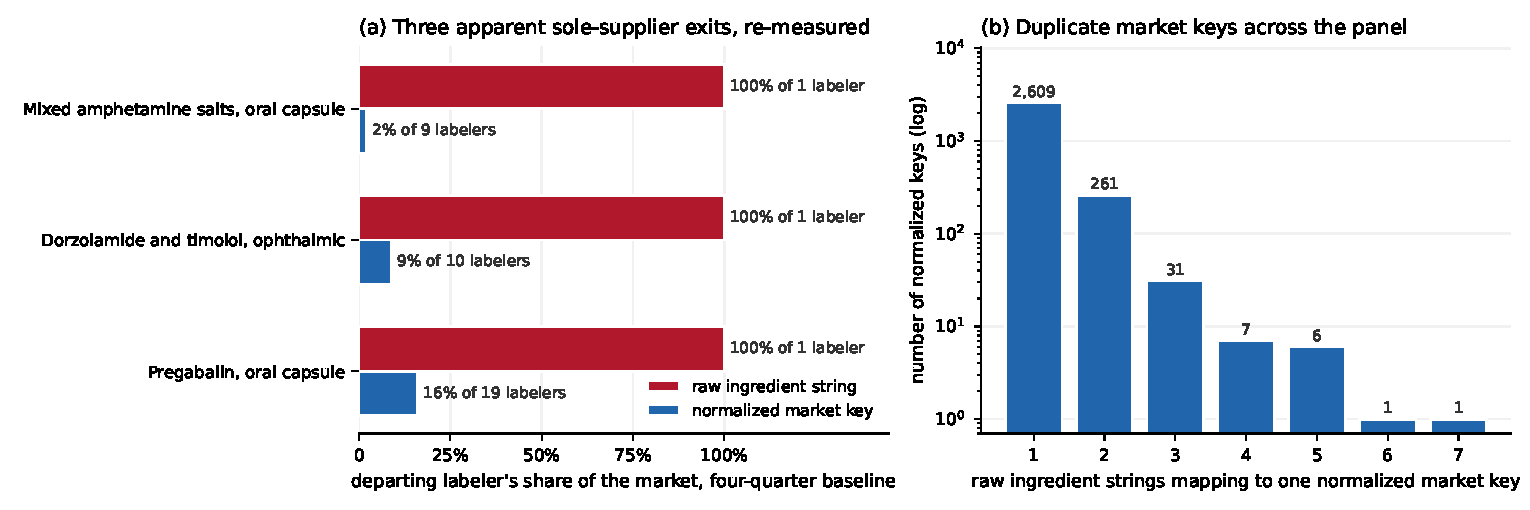
\includegraphics[width=\textwidth]{fig1.pdf}
\caption{(a) Three exits recorded by the raw specification as the departure of a market's only
supplier, re-measured on the corrected market key. (b) How many raw ingredient strings map to
each normalised key across the panel; the vertical scale is logarithmic.}\label{fig:defect}
\end{figure}

\subsection{The merges are confirmed by independent ingredient data}\label{subsec:validres}

Of 333 merge groups covering 757 raw keys, 316 are testable against FDA substance data. The
substance data confirms 305 and contradicts 11, a precision of 96.5 percent; 17 groups are not
testable because substance names are missing for every member. Of the 11 contradicted groups,
most reflect FDA's own naming of hydrates rather than a false merge, with paroxetine recorded
both as paroxetine and as paroxetine hemihydrate and darunavir both as darunavir and darunavir
hydrate. One is a genuine residual failure: Trace Elements 4 and Trace Elements 5 differ in the
number of elements they contain and our rule, which discards bare numerals, merges them.

The opposite error also exists. Searching for distinct normalised keys that share a substance
set and a route bucket finds groups the algorithm did not merge, which means the normalisation
is conservative and the 424 figure is a lower bound on the number of duplicate keys in these
data.

We report this check as supportive rather than decisive. Both fields come from FDA product
listings and share an upstream source, so agreement between them is weaker evidence than
agreement with an external terminology would be. RxNorm would supply that, and we could not
reach it from the analysis environment.

\subsection{What actually caused each sole-labeler exit}\label{subsec:causeres}

Table~\ref{tab:cause} classifies all thirteen remaining sole-labeler exits against public
records. Three are not supply disruptions. Ranitidine was removed from the US market altogether
at FDA's request in April 2020 after nitrosamine contamination was found to increase during
storage, so no replacement by other labelers was possible or desirable. Alcaftadine and
olopatadine ophthalmic solutions left the prescription market through approved
prescription-to-over-the-counter switches; dispensing did not stop, it moved off the Medicaid
pharmacy benefit. In all three the absence of replacement is the intended outcome of a
regulatory action, and reading it as a failure of market resilience inverts its meaning.

Three are documented supply disruptions, and they are not three independent episodes. Diclofenac
potassium tablets entered the ASHP shortage record in February 2019 with Teva, the departing
labeler here, named and offering no public reason; the exit falls inside that shortage.
Varenicline accounts for the other two, both exits by Pfizer in the quarters during which it
recalled all lots of the product for nitrosamine content and FDA acknowledged a resulting
shortage. Those two are one disruption affecting two formulations, so the verified-supply
stratum rests on two episodes, not three events, and we treat it accordingly throughout.

Seven exits could not be classified. Several are small multivitamin, prenatal and combination
otic products of the kind whose withdrawal is more often commercial than operational, but we did
not find records sufficient to say so, and we do not.

\begin{table}[htbp]
\caption{Every sole-labeler exit in the analysis cohort, with its classification against public
records and its replacement ratio. Markets are named by ingredient and route-and-form
bucket.}\label{tab:cause}
\begin{tabular}{@{}llllr@{}}
\toprule
Quarter & Market & Departing labeler & Classification & $R$ \\
\midrule
2018Q2 & Multivitamin with minerals, oral tablet & BonGeo & undetermined & 0.00 \\
2018Q3 & Iron, folic acid, vitamin, other        & Women's Choice & undetermined & 0.00 \\
2019Q3 & Hydrocortisone and acetic acid, otic    & Sun   & undetermined & 0.00 \\
2019Q3 & Diclofenac potassium, oral tablet       & Teva  & supply disruption & 0.00 \\
2020Q2 & Ranitidine, oral tablet                 & Amneal & non-supply: withdrawal & 0.00 \\
2021Q2 & Brinzolamide and brimonidine, ophthalmic & Alcon & undetermined & 0.00 \\
2021Q3 & Olopatadine, ophthalmic                 & Alembic & non-supply: OTC switch & 0.00 \\
2021Q3 & Varenicline, other                      & Pfizer & supply disruption\textsuperscript{a} & 0.24 \\
2021Q4 & Varenicline, oral tablet                & Pfizer & supply disruption\textsuperscript{a} & 0.69 \\
2021Q4 & Goserelin, injectable                   & TerSera & undetermined & 0.00 \\
2022Q1 & Trimethoprim, oral tablet               & Lupin & undetermined & 0.08 \\
2022Q2 & Alcaftadine, ophthalmic                 & Allergan & non-supply: OTC switch & 0.00 \\
2023Q3 & Griseofulvin, oral liquid               & Cipla & undetermined & 0.00 \\
\botrule
\end{tabular}
\footnotetext[1]{The two varenicline exits are the same recall episode affecting two
formulations, not independent disruptions.}
\end{table}

One consequence of doing this properly is worth recording. An earlier version of this analysis
matched recalls to events at the ingredient level and found a recall flag contemporaneous with
fourteen of twenty sole-labeler exits. Matching instead on the departing labeler and its own
exit quarter, as causal attribution requires, leaves one: Pfizer's varenicline recall. The
ingredient-level association was an artefact of matching on a shared ingredient rather than on
the firm that left.

\subsection{Replacement falls with the departing share}\label{subsec:replace}

Table~\ref{tab:R} reports replacement on the corrected panel. Where the departing labeler held
under 35 percent of the market, the remaining labelers took up roughly 1.8 times what left,
which reflects both substitution and background growth; where it held 65 to 95 percent they took
up about four fifths; where it held at least 95 percent the median market took up nothing. Ten
of thirteen sole-labeler markets have a replacement ratio under 0.02.

The ordering is not strictly monotone. The 35-to-65 percent band holds three markets and a
negative median, which is a feature of three observations rather than a finding; we draw no
inference from it and describe the pattern as a contrast between the extreme bands.

\begin{table}[htbp]
\caption{Replacement ratio by the departing labeler's pre-exit share. Intervals are percentile
bootstrap intervals for the median over 20{,}000 resamples. The final two columns are different
endpoints and are not comparable to one another: $R<0.02$ counts markets where the other
labelers did not expand, collapse counts markets whose own dispensing fell below two percent of
baseline.}\label{tab:R}
\begin{tabular}{@{}lrrrrrrr@{}}
\toprule
Departing share & $n$ & Median $R$ & 95\% CI & Mean & Vol-wtd & $R<0.02$ & Collapse \\
\midrule
under 35 percent    & 77 & 1.77 & [1.11, 2.49]   & 19.29 & 14.63 & 27.3\% & 0.0\% \\
35 to 65 percent    & 3  & $-0.13$ & [$-1.09$, 1.48] & 0.09 & 1.17 & 66.7\% & 0.0\% \\
65 to 95 percent    & 6  & 0.82 & [0.37, 1.13]   & 0.77  & 0.90  & 0.0\%  & 0.0\% \\
at least 95 percent & 13 & 0.00 & [0.00, 0.00]   & 0.08  & 0.31  & 76.9\% & 38.5\% \\
\botrule
\end{tabular}
\end{table}

The mean in the lowest band is far above its median, reflecting a long right tail: when a small
labeler leaves a growing market, unrelated growth by the others produces a very large ratio. The
volume-weighted figure of 14.63 in that band is dominated by a handful of large growing markets
and should be read as a description of where the volume sits, not as a typical market's
behaviour. The median is the appropriate summary.

\begin{figure}[htbp]
\centering
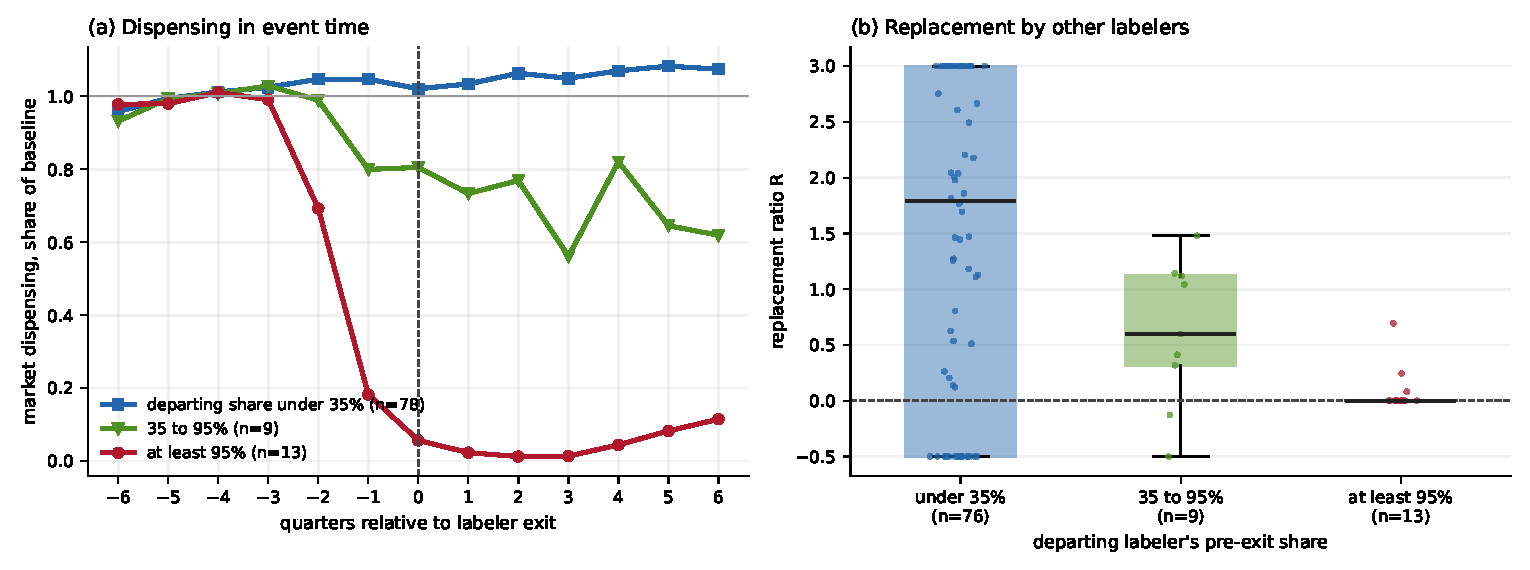
\includegraphics[width=\textwidth]{fig2.pdf}
\caption{(a) Median market dispensing in event time as a share of baseline, by the departing
labeler's prior share. (b) Replacement ratios by band; points are individual markets, boxes show
the interquartile range and median, and values are clipped to the plotted range. Unclipped
event-level values are released with the paper.}
\label{fig:eventtime}
\end{figure}

\subsection{Comparison with matched controls}\label{subsec:matched}

Five of the thirteen sole-labeler markets, 38.5 percent, collapse below two percent of baseline
dispensing. Among 325 matched risk-set control observations, none does. The matched risk
difference is 38.5 points, with a 95 percent interval of 15.4 to 61.5 points when whole matched
sets are resampled. An interval that additionally resamples controls within each set is
identical, because the control collapse rate is zero in every set and so contributes no
variance; all of the uncertainty comes from the thirteen treated events, and the interval should
be read in that light.

Two weaknesses are worth stating rather than asserting away. First, control eligibility requires
that a market have no detected exit at or before $t+6$, which uses information from after $t$. A
strict risk set would condition only on information available at $t$; we use the forward-looking
rule because a market that loses a labeler two quarters later is not a clean counterfactual for
the six-quarter outcome window, and we note that the choice makes the control group cleaner and
therefore the contrast larger than a strict risk set would. Second, because a good control must
itself contain a labeler with a near-total share and must not be exposed, only 39 distinct
markets qualify across all thirteen matched sets. Five appear once; one appears in all thirteen.
The 325 control observations are far from 325 independent markets. The contrast between 38.5
percent and zero is large, but it rests on a thin and heavily reused comparison group, and the
honest reading is that markets structurally similar to the treated ones are scarce in these data
precisely because near-sole-supplier markets are scarce.

\subsection{The result does not hold in the events we can verify}\label{subsec:strata}

Table~\ref{tab:strata} stratifies replacement by the classification in Table~\ref{tab:cause}.
Removing the three verified non-supply events, the minimum correction any supply-chain
interpretation requires, leaves the median at zero. But the three events in which a supply
disruption is documented have a median replacement ratio of 0.24, and only one of the three
collapses. The zero-replacement result is carried by the seven events whose cause we could not
establish, where the median is zero and six of seven have a replacement ratio under 0.02.

\begin{table}[htbp]
\caption{Replacement among sole-labeler exits, by what the exit is verified to be. The
documented-disruption row covers three events arising from two episodes, since the two
varenicline exits are one recall.}\label{tab:strata}
\begin{tabular}{@{}lrrrr@{}}
\toprule
Stratum & $n$ & Median $R$ & $R<0.02$ & Volume-weighted $R$ \\
\midrule
All sole-labeler exits                      & 13 & 0.00 & 76.9\% & 0.31 \\
Excluding verified non-supply events        & 10 & 0.00 & 70.0\% & 0.38 \\
\quad of which documented supply disruption & 3  & 0.24 & 33.3\% & 0.46 \\
\quad of which cause undetermined           & 7  & 0.00 & 85.7\% & 0.01 \\
Verified non-supply events                  & 3  & 0.00 & 100.0\% & 0.00 \\
\botrule
\end{tabular}
\end{table}

Three events from two episodes cannot settle anything, and we do not claim the difference
between the strata is estimable. A median replacement ratio of 0.24 is not evidence of
successful recovery either; it says that about a quarter of the departing volume was taken up.
What the table establishes is a negative: this panel does not support the statement that
sole-supplier markets fail to replace lost volume after a supply disruption, because in the
events where a supply disruption is documented, part of it was replaced. The pattern is
consistent with a mechanism worth testing on a larger sample, that a documented shortage draws
expansion from remaining suppliers while a quiet commercial exit from a thin market draws none,
but this panel cannot test it.

\subsection{Recovery, measured from the first decline}\label{subsec:recovery}

Markets with twelve observed quarters after the exit form a longitudinal cohort of 76, of which
58 are minority-loss, 6 middle and 12 sole-labeler. We measure recovery from each market's first
crossing below a threshold rather than from the exit, because the at-risk population otherwise
changes with the horizon: a market first falling below 90 percent of baseline in quarter eleven
would enter a twelve-quarter comparison with one quarter in which to recover.

Of the minority-loss markets, eight ever fall below half of baseline and five of those recover;
all twelve sole-labeler markets fall below half and six recover. The log-rank comparison of time
to restoration gives $p=0.194$. At the 90 percent threshold, 28 minority-loss markets cross and
13 recover, against 12 of 12 crossing and 3 recovering among sole-labeler markets, with
$p=0.056$. A landmark analysis restricted to markets crossing within four quarters of the exit
gives 5 of 6 against 6 of 12 at the 50 percent threshold and 12 of 22 against 3 of 12 at the 90
percent threshold.

\begin{figure}[htbp]
\centering
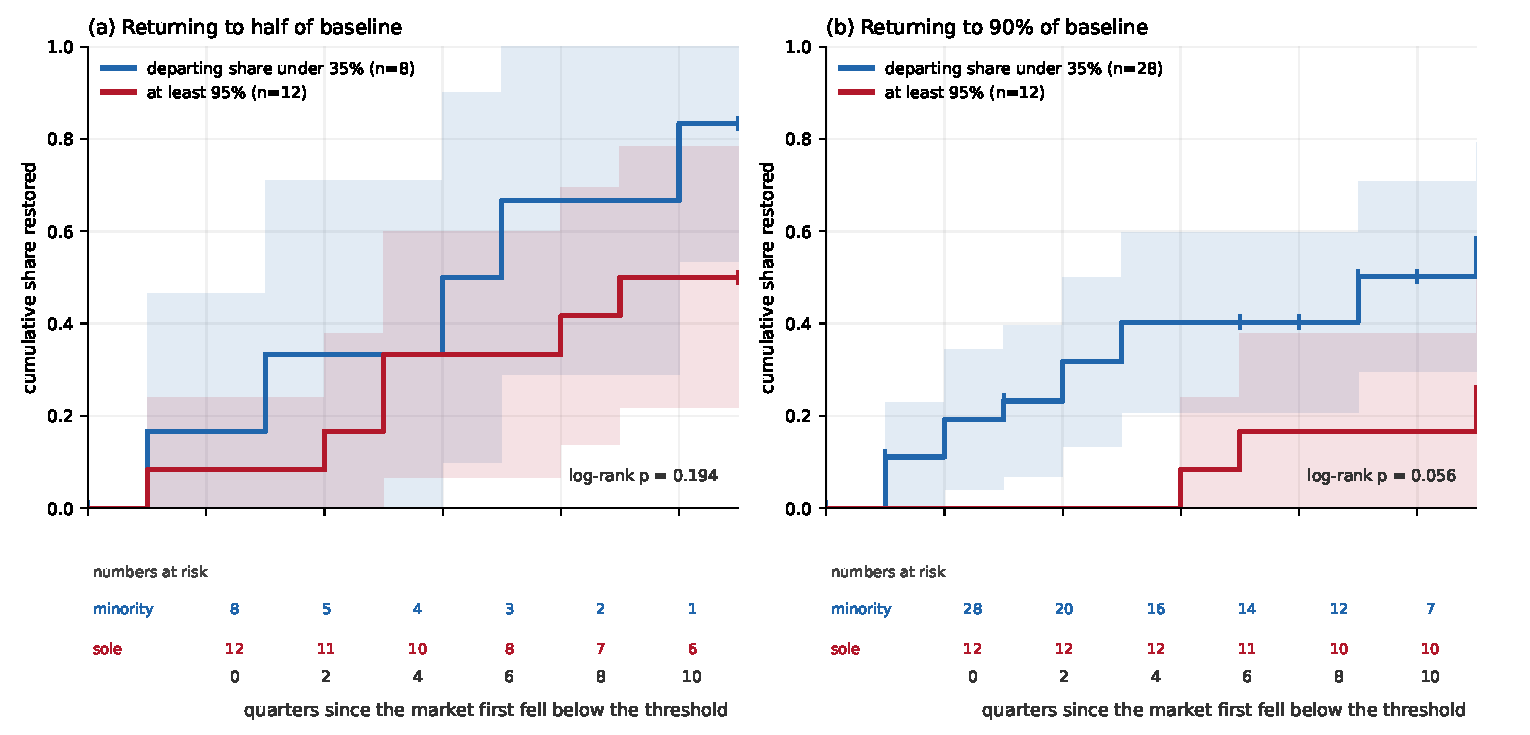
\includegraphics[width=\textwidth]{fig3.pdf}
\caption{Cumulative share of markets restored to (a) half and (b) 90 percent of baseline
dispensing, measured from each market's first crossing below that threshold, with markets never
restored censored at the end of follow-up. Tick marks denote censoring.}\label{fig:recovery}
\end{figure}

Two things follow. The difference in whether a market falls at all is stark: every sole-labeler
market in this cohort falls below half of baseline, against eight of 58 minority-loss markets.
The difference in whether a fallen market comes back is suggestive at the 90 percent threshold
and not established at the 50 percent threshold. We report $p=0.056$ as suggestive and
specifically not as a demonstrated effect. We note that the previous, fixed-horizon version of
this analysis returned $p=0.206$ for the same comparison; the censored design is the correct one
and it happens to be the more favourable one, which is a reason to state plainly that we adopted
it on methodological grounds before seeing that result.

\subsection{Cumulative unreplaced dispensing}\label{subsec:deficit}

Summing the per-quarter shortfall against baseline over twelve quarters, and expressing it in
quarters of baseline volume, gives a median total deficit of 0.2 quarters where the departing
share was under 35 percent, 5.6 where it was 35 to 95 percent, and 10.4 where it was at least 95
percent. Restricting to quarters $t+4$ onward, outside the four-quarter window used to detect the
event, the medians are 0.0, 3.8 and 6.6 quarters, with a bootstrap interval of 3.7 to 8.0 for the
sole-labeler band and a leave-one-out range of 5.5 to 7.8. Each figure is a separately computed
median over event-level deficits, not a sum of component medians.

\subsection{Entry}\label{subsec:entry}

A new labeler dispenses within six quarters in 74.1 percent of minority-loss markets, 33.3
percent of middle markets and 33.3 percent of sole-labeler markets. We count any labeler not
previously dispensing in that market, which includes relabeling and the return of a firm that had
paused, so this is an upper bound on genuine entry.

\subsection{Labelers overstate manufacturing redundancy}\label{subsec:estab}

Structured Product Labeling records list, for each labeled product, the establishments registered
to manufacture, analyse or supply the active ingredient for it \cite{dailymed}. Pooling
establishments across a labeler's whole portfolio, which is the natural thing to do when working
from labeler identifiers alone, attributes about four establishments to a typical departing
labeler. Restricting to the establishments listed for the specific products that were actually
dispensing in the market reduces this to roughly one, with most sole-labeler markets resting on a
single listed site. This is a second route to the same conclusion as
Section~\ref{subsec:defect}: counts taken at a convenient level of aggregation overstate
redundancy, and the overstatement runs in the direction that makes markets look safer than they
are. A limitation applies: these listings describe current labels, not the labels in force at the
time of each exit, so they characterise the products rather than reconstruct their history.

\subsection{Robustness}\label{subsec:robust}

Table~\ref{tab:flow} already reports the three specifications end to end. On the headline
quantities, the raw convention gives a sole-labeler median replacement ratio of 0.00 with 80.0
percent of markets below $R=0.02$ and a collapse rate of 45.0 percent on twenty events;
correcting the route bucketing alone changes neither; correcting the ingredient key as well
gives 0.00, 76.9 percent and 38.5 percent on thirteen events. The minority band moves from 1.58
to 1.77. The direction and the ordering of the extreme bands are unchanged, so the corrections
repair the event classification without manufacturing the contrast. We report the two endpoints
separately throughout because they answer different questions and differ substantially: 76.9
percent of sole-labeler markets saw no expansion by other labelers, while 38.5 percent lost
nearly all of their own dispensing.

Suppression remains a source of uncertainty we cannot eliminate. The withholding rule covers
records under eleven prescriptions, but CMS also applies secondary suppression, so assigning a
maximum of ten prescriptions to each withheld record is a working assumption and not a proven
bound. Treating every suppressed post-event record as carrying ten prescriptions moves one
market's classification, and we report the complete-case rate and that scenario as two figures
rather than resolving them into one. Separately, markets with no observed post-event quarter are
dropped rather than coded as collapsed; coding them as collapsed would raise the sole-labeler
collapse rate and coding them as surviving would lower it, and we report the complete-case
figure with that range stated rather than choosing.

\section{Discussion}\label{sec:discussion}

The count of single-source drug markets is a policy object. It appears in regulatory root-cause
analysis, in arguments for reshoring and stockpiling, and in proposals to subsidise redundancy.
This paper shows that in the most widely used public dispensing data the count is inflated by
two defects that operate before any supplier is counted. The market is identified by a dosage
form that does not record where the product acts, so eye drops, ear drops, topical solutions and
oral syrups sharing an ingredient are pooled; and it is named by an unnormalised free-text
string, so one product occupies several keys. Thirteen percent of keys are duplicates of
another, and the duplicates concentrate in exactly the configuration that generates a false
positive: a rarely used spelling that one labeler happens to favour becomes a market with one
supplier in it. Six of twenty apparent sole-supplier exits in this panel are not sole-supplier
exits.

This complements rather than contradicts Colazo \cite{colazo2026}, whose concern is that
supplier counts record administrative visibility rather than operational redundancy. The two
errors compound. A count can be wrong because the firms it counts do not represent independent
capacity, and it can be wrong because the market it counts is a fragment of a larger market. Our
establishment analysis in Section~\ref{subsec:estab} reproduces the first error from a different
direction; Section~\ref{subsec:defect} documents the second. That the raw procedure reproduces
Colazo's market count to within two of 3{,}344 suggests the second error is present wherever this
market definition is used on these data. We emphasise that this is a defect in a shared
procedure, not in that paper's argument, which our results support.

The second contribution is less comfortable. Having repaired the market definition, we audited
what the surviving events actually were, and three of thirteen turned out to be regulatory
rather than operational. The removal of ranitidine from the US market is the clearest: a market
in which no supplier replaced the departing one, because the agency had asked all of them to
leave. An analysis that reads zero replacement as a failure of supply-chain resilience records
the regulatory system working as intended as evidence that it is broken. The two
prescription-to-over-the-counter switches are subtler and, for Medicaid dispensing data
specifically, more dangerous, because the product remains available and the dispensing merely
moves off the benefit; nothing in the panel distinguishes that from a product vanishing.

The implication is methodological and it generalises beyond this paper. Where an event study is
built on administrative dispensing data, the event must be validated against records outside the
series that defines it. Our own earlier attempt to do this by matching recalls at the ingredient
level produced a contemporaneous recall flag for fourteen of twenty events; matching on the firm
that actually departed produced one. The first number would have supported a supply-side reading
and it was an artefact of matching on a shared ingredient rather than on the exiting firm.

What survives both corrections is a robust association. Pre-exit concentration predicts whether
a market loses its dispensing: replacement ratios fall from 1.77 at the low end to 0.00 at the
high end, every sole-labeler market in the longitudinal cohort falls below half of baseline
against eight of 58 minority-loss markets, and the matched comparison puts the collapse rate at
38.5 percent against zero. Whether a fallen market returns is a separate question, and on the
correct censored design the answer is suggestive at the 90 percent threshold and not established
at the 50 percent threshold.

The finding we did not expect is that the zero-replacement result is concentrated in the events
we could not explain. Where a shortage is documented and the departing firm is named in it,
replacement is partial: a median ratio of 0.24 across three events arising from two episodes. We
are explicit that this supports no estimate. But the direction matters for how the literature should read results
of this kind, because it is the opposite of what a supply-resilience interpretation predicts, and
the events that do produce the predicted pattern are small, low-value products of the kind that
leave quietly. A plausible reading is that a documented shortage is itself a signal that draws
expansion from remaining suppliers, while an unannounced commercial exit from a thin market draws
none. That is a hypothesis this panel raises and cannot test.

\subsection{Limitations}

The sample of sole-labeler exits cannot be enlarged within these data. Thirty-nine exist in the
panel; twenty fall outside a window that a forty-one quarter panel with six quarters of history
and six of follow-up necessarily imposes, and six have every post-event quarter suppressed. No
choice of baseline rule recovers them. Any analysis of sole-supplier exits in SDUD over this
period is working with on the order of a dozen events, and conclusions drawn from strata of such
a sample are descriptive.

Medicaid dispensing is not total US dispensing. A product that leaves the Medicaid benefit while
remaining available elsewhere looks identical here to a product that leaves the market, which is
exactly the failure mode the over-the-counter switches illustrate. We addressed this by
classifying events against external records rather than by assuming it away, but the classification
rests on what is publicly documented, and absence of a shortage record is weak evidence of
absence of a shortage, particularly before the current FDA database retention practices.

The outcome is dispensing, not unmet clinical need. A market whose volume does not return may
have been appropriately abandoned in favour of a better therapy. We cannot distinguish that from
patients going without, and we do not claim to.

The establishment linkage describes current labels rather than the labels in force at each exit.
A version-history reconstruction would strengthen it and is the clearest extension of this work.

\section{Conclusion}\label{sec:conclusion}

Before asking how many suppliers a drug market has, it is worth asking whether the market is a
market. In a decade of national Medicaid dispensing data, the standard
ingredient-by-dosage-form convention identifies markets by a form field that does not record
route, and names them with an unnormalised string of which 424 of 3{,}294 keys are duplicates of
another. Repairing both dissolves six of twenty apparent sole-supplier exits, in one case
converting a firm with 6.4 percent of a nineteen-supplier market back from being that market's
only supplier. Of the thirteen that survive the repair, three are regulatory actions rather than
supply failures.

What remains is a clear association between pre-exit concentration and the loss of a market's
dispensing, robust to both corrections, together with a caution about what it means. In the three
events from two episodes where a supply disruption is actually documented, remaining suppliers
replaced part of the lost volume. The strong form of the single-source resilience claim, that such markets do not
recover after a supply disruption, is not what these data show once the events are verified.

For researchers using these data, four practices follow: bucket markets by route of
administration and not by dosage form alone, normalise the ingredient key before counting
suppliers and validate the merges against structured ingredient data, validate events against
records outside the dispensing series, and report events of undetermined cause as their own
stratum rather than assuming them into the hypothesis under test. For policy, the count of single-source markets drawn from public dispensing data
should be treated as an upper bound, and the subset of it that reflects genuine operational
fragility is smaller than the raw figure implies.

\backmatter

\section*{Declarations}

\textbf{Funding.} No funding was received for this work.

\textbf{Conflicts of interest.} The authors declare no competing interests.

\textbf{Ethics approval.} Not applicable. The study uses only publicly released aggregate data
and involves no human subjects.

\textbf{Data availability.} All data are public: Medicaid State Drug Utilization Data
\cite{cms_sdud}, the FDA National Drug Code Directory \cite{fda_ndc}, openFDA datasets
\cite{openfda}, the FDA drug shortage database \cite{fda_shortages} and DailyMed Structured
Product Labeling \cite{dailymed}.

\textbf{Code availability.} The panel construction, the market-key normalisation map, the
event-level cohort manifest and the event cause classification are released with the paper, so
that every number above can be recomputed and every event-level classification inspected.

\textbf{Author contributions.} V.A. designed the study, built the data pipeline, performed the
analysis and wrote the manuscript. S.K. contributed to the clinical interpretation of the
affected products and reviewed the manuscript.

\bibliographystyle{sn-vancouver-num}
\bibliography{refs}

\end{document}
